\documentclass[12pt]{article}
\usepackage[margin=0.8in]{geometry}
\usepackage[utf8]{inputenc}
\usepackage{tikz}
\usepackage{graphicx}
\usepackage{amsmath}
\usepackage[version=4]{mhchem}
\usepackage{siunitx}
\usepackage{longtable,tabularx}
\usepackage{cleveref}
\setlength\LTleft{0pt} 
\usepackage{subcaption}
\usepackage{relsize}
\usepackage{float}
\usepackage{booktabs}
\usepackage{bm}
\usepackage{comment}
\graphicspath{ {./Figures/} }
\usepackage{amssymb}
\usepackage{listings}
\usepackage{color} %red, green, blue, yellow, cyan, magenta, black, white
\definecolor{mygreen}{RGB}{28,172,0} % color values Red, Green, Blue
\definecolor{mylilas}{RGB}{170,55,241}

\date{} 
\title{Project 2 \large \\
        Statistical Patter Recognition}

\author{Girguis Sedky} 
\begin{document}
\maketitle

%---------------------------------------------------------------------------------------------
\section{Support Vector Machine}
In this method, we use train a support vector machine (SVM) on the training FMNIST data, which consists of 60,000 images of 10 different clothing items and deploy the trained algorithm on the test data, which consists of 10,000 images. LIBSVM was used here. The dimension of the image vectors are reduced from $28*28=784$ to $50$ dimensions using principal component analysis before the training procedure. We try three different Kernels, including a linear kernel, a third degree polynomial kernel, and a radial basis function kernel (RBF). Figure~\ref{fig:SVM} shows a comparison of the accuracy of the SVM algorithm in classifying the test data with each kernel. All of the algorithms do relatively well. The SVM algorithm trained using the RBF kernel is the most accurate classifier. 


\begin{figure}[h]
 \centering
  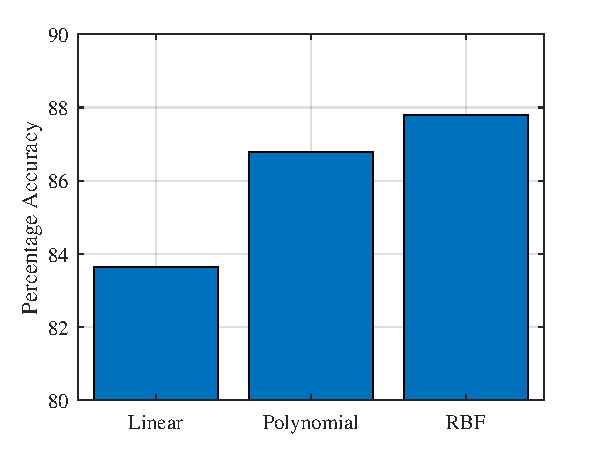
\includegraphics[width=0.7\linewidth]{SVM_Accuracy.pdf}
  \caption{Bayesian classifier}
  \label{fig:SVM}
\end{figure}

%----------------------------------------------------------------------------------
\section{Convolutional Neural Network}
In this section, we utilize a CNN to classify the test images. No PCA is performed o the data set that is used here. The network used is a variant on LeNet that is shown in Fig.~\ref{fig:NN}. It consists of 7 layers and an alternating convolution and max pooling application from one layer to the next. ReLU is introduced in the final transition layer. MatCovNet toolbox was utilized to develop, train, and implement this neural network.  
\begin{figure}[H]
 \centering
  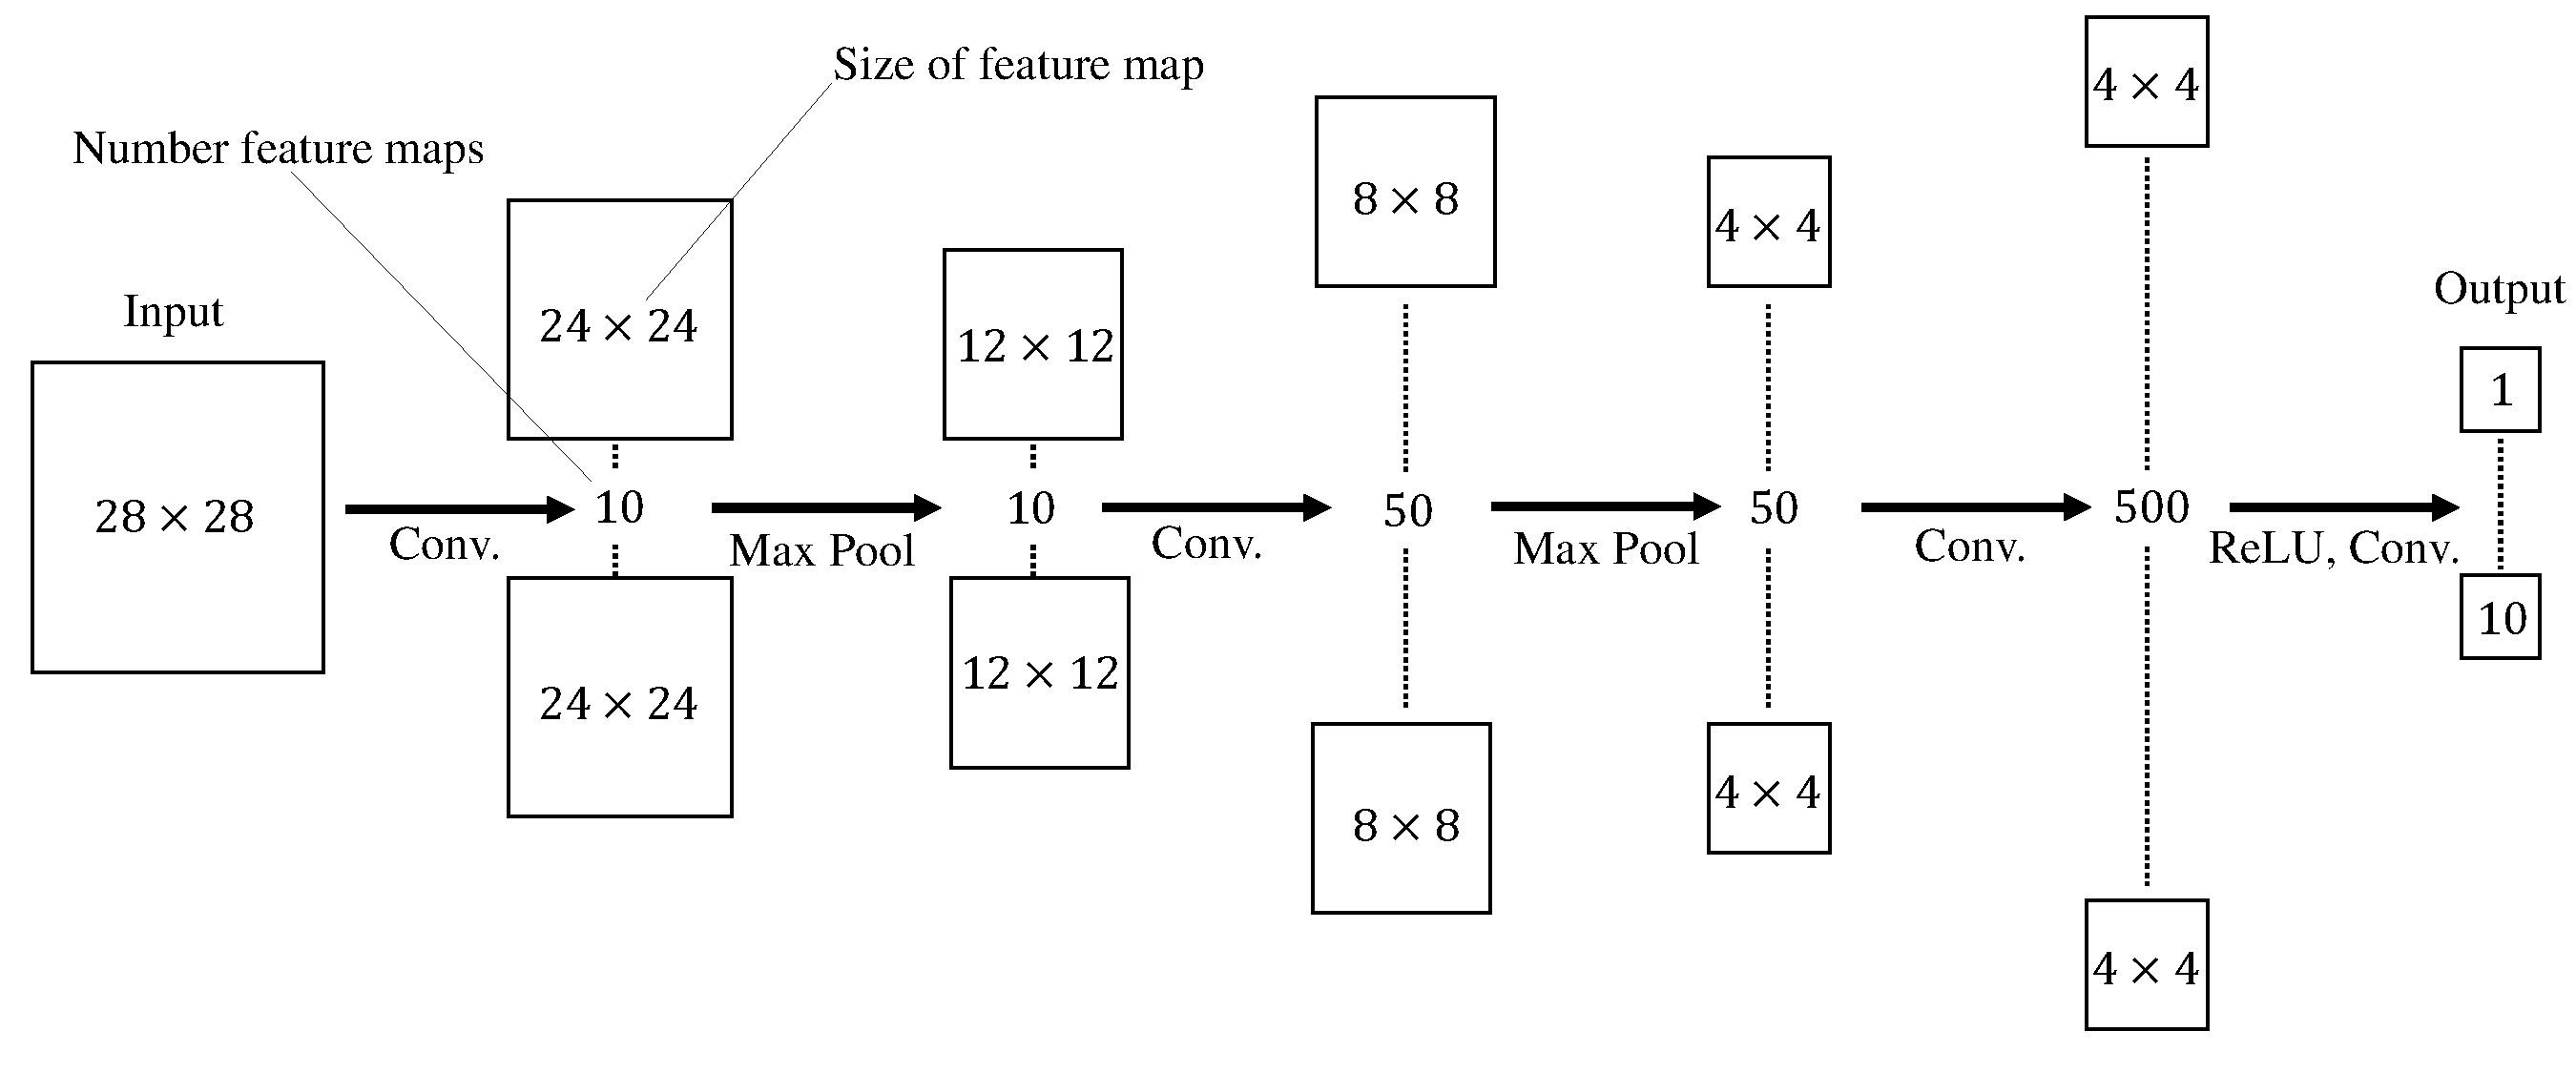
\includegraphics[width=\linewidth]{NN.pdf}
  \caption{Convolutional Neural Network layout}
  \label{fig:NN}
\end{figure}
The data is divided into batches of 100 images, and the network goes through the entire data set 15 times (15 epochs) during the gradient descent procedure to tune all the weights. Figure~\ref{fig:Error} shows the rate of descent of error as a function of the epoch number. The error rate has a steep drop during the first couple of passes through the data, and then its continues decreasing with a steadier pace. The trained CNN is able to classify the test images with 90.6\% accuracy which is a higher accuracy compared to SVM. This improvement in accuracy can be attributed to the increased complexity of the classifier, large number of empirical weights that can be tuned in training, and non-linearity introduced by the ReLU operator. 
\begin{figure}[H]
 \centering
  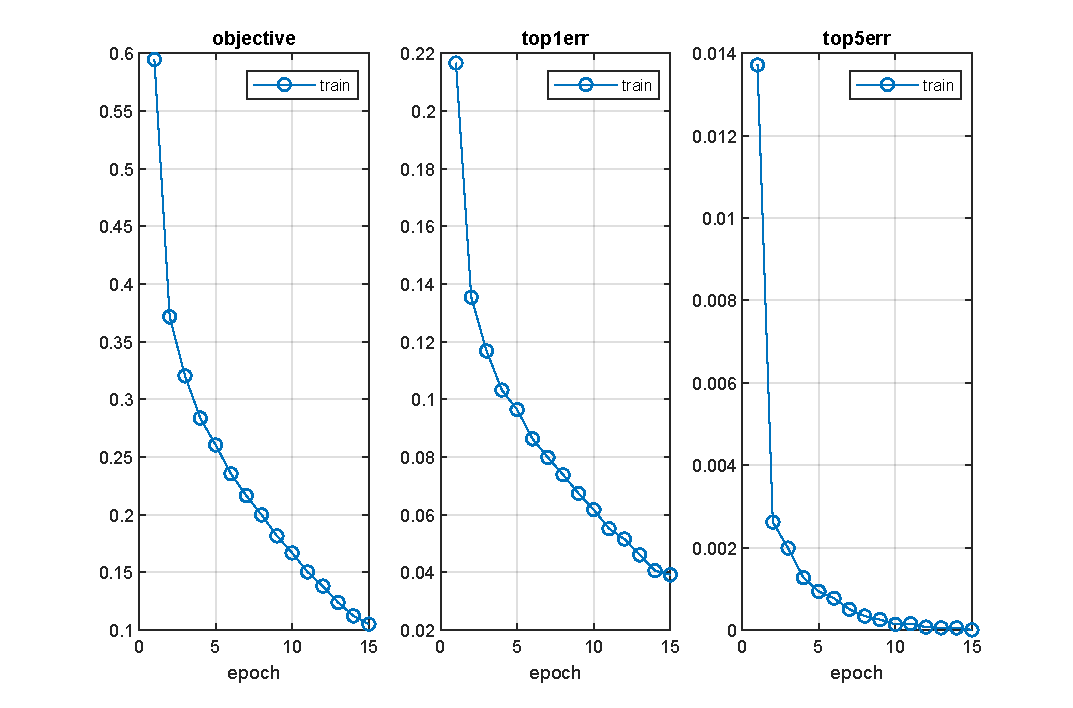
\includegraphics[width=\linewidth]{Error.pdf}
  \caption{The descent rate of error in classifying the training data}
  \label{fig:Error}
\end{figure}

%----------------------------------------------------------------------------------------------
\section{Summary}
Table~\ref{table:1} shows the classification error of the different methods utilized in project 1 and 2. In Project 1, the most accurate method of classification was to use principal component analysis to reduce the conventionality of the state vectors to 50 and then to apply Nearest-Neighbor (NN) classification to the transformed data.

In this project, both Support Vector Machines (SVM) and Convolutional Neural Networks (CNN) were superior in performance to all the methods used in project 1. CNN proves to be the best classifier. This can be attributed to the increased complexity of the classifier, large number of empirical weights that can be tuned in training, and non-linearity introduced by the ReLU operator. 
\begin{table}[H]
\centering
\caption{Summary of classification results}
\label{table:1}
\begin{tabular}{cc}
\hline
Method     & Percentage Error \\ \hline
SVM (RBF Kernel)      & 12\%  \\
CNN         & 9.39\%          \\
Bayes      & 35\%             \\
NN         & 15\%             \\
PCA, Bayes (50) & 20.5\%      \\
PCA, NN  (150)  & 14.7\%      \\
LDA, Bayes & 25.4\%           \\
LDA, NN    & 28\%             \\ \hline
\end{tabular}
\end{table}

%----------------------------------------------------------------------------------
% Appendix Matlab code
\lstset{language=Matlab,%
    %basicstyle=\color{red},
    breaklines=true,%
    morekeywords={matlab2tikz},
    keywordstyle=\color{blue},%
    morekeywords=[2]{1}, keywordstyle=[2]{\color{black}},
    identifierstyle=\color{black},%
    stringstyle=\color{mylilas},
    commentstyle=\color{mygreen},%
    showstringspaces=false,%without this there will be a symbol in the places where there is a space
    numbers=left,%
    numberstyle={\tiny \color{black}},% size of the numbers
    numbersep=9pt, % this defines how far the numbers are from the text
    emph=[1]{for,end,break},emphstyle=[1]\color{red}, %some words to emphasise
    %emph=[2]{word1,word2}, emphstyle=[2]{style},    
}

\newpage
\section*{Appendix}
\subsection*{SVM}
\subsubsection*{PCA}
\lstinputlisting{Scripts/PCA.m}
\newpage
\subsubsection*{Training script}
\lstinputlisting{Scripts/TrainSVM.m}
\newpage
\subsubsection*{Testing script}
\lstinputlisting{Scripts/TestSVM.m}
\newpage
\subsection*{CNN}
\subsubsection*{Neural network initialization}
\lstinputlisting{Scripts/initialize_FMNIST_CNN.m}
\newpage
\subsubsection*{Main training and testing script}
\lstinputlisting{Scripts/CNN_FMNIST_Script.m}

\end{document}